\documentclass{article}

% Language setting
% Replace `english' with e.g. `spanish' to change the document language
\usepackage[english]{babel}

% Set page size and margins
% Replace `letterpaper' with `a4paper' for UK/EU standard size
\usepackage[letterpaper,top=2cm,bottom=2cm,left=3cm,right=3cm,marginparwidth=1.75cm]{geometry}

% Useful packages
\usepackage{amsmath}
\usepackage{graphicx}
\usepackage[colorlinks=true, allcolors=blue]{hyperref}

\title{Bezier Curves}
\author{Stan Laguerre Mila Zhou Ben Crotteau}

\begin{document}
\maketitle

\begin{abstract}
This paper explores the use of Bezier curves in designing fonts. Bezier curves are made up of cubic splines, and give the user control over the shape of these functions. This makes Bezier curves more suited for letter design than normal cubic splines that prioritize the smoothness of the first and second derivatives of the graph over its shape. Designing letters takes a significant amount of information as 4 points are needed to make any given curve on the graph, but once they are complete, they can be coded into a function and called at the user's desire. This paper describes the properties of Bezier curves, gives examples of three different letters created using them, and gives helpful tips for this process.
\end{abstract}

\section{Introduction}

Bezier curves are a specific type of cubic spline that are used in computational mathematics to approximate functions and fit data. Cubic splines are a type of data fitting that fits a cubic function between two successive points in a plot. The key difference between Bezier curves and typical cubic splines is the slope at the endpoints. Typical cubic splines seek to have a continuous first and second derivative at each point between neighboring splines to have a smooth curve. Bezier curves give the user control over the slope at the end points of each spline, so it can differ at the endpoints that are connected to two different splines potentially resulting in sharp points. This user control makes Bezier curves better suited for font design than typical cubic splines.

\section{Bezier Curve Letter Design}

\subsection{Bezier Curves}

Bezier curves are comprised of cubic splines between two endpoints with the slope at the endpoints determined by control points. The endpoints are simply the beginning and end of the Bezier curve. The control points impact the slope at the endpoints. The slope between the endpoint and the control point is set to be the slope at the endpoint. This is achieved by setting the derivative of the cubic spline equal to the difference between the control point and endpoint at the beginning, and the difference between the endpoint and control point at the end. 

Thus, each spline in a Bezier curve has 4 points: 2 endpoints and 2 control points. Because the slope at the endpoints is determined by the control points, a Bezier curve with connected splines may not be smoothness of the first and second derivative and we may get sharp corners.

To understand the nuts and bolts of how Bezier curves work, take the example of the single Bezier curve. A single Bezier curve is a parametric equation where:

$$
b(t) = (x(t),y(t))
$$
$$
x(t) = x_1 + b_x t + c_x t^2 + d_x t^3
$$
$$
y(t) = y_1 + b_y t + c_y t^2 + d_y t^3
$$
$$
0 \leq t \leq 1
$$

These equations meet the following properties: $x(0) = x_1$, $x'(0) = 3(x_2-x_1)$, $x'(1) = 3(x_4-x_3)$, $x(1) = x_4$, $y(0) = y_1$, $y'(0) = 3(y_2 - y_1)$, $y'(1) = 3(y_4-y_3)$, $y(1) = y_4$. Solving with these properties, we get:

$$
b_x = 3 (x_2 - x_1)
$$
$$
c_x = 3(x_3 - x_2) - b_x
$$
$$
d_x = x_4 - x_1 - b_x - c_x
$$
$$
b_y = 3 (y_2 - y_1)
$$
$$
c_y = 3(y_3 - y_2) - b_y
$$
$$
d_y = y_4 - y_1 - b_y - c_y
$$

These are simple formulas to code, and repeating this process for multiple collections of 4 points will get multiple Bezier curves. If the endpoints match for these different curves, then they will be connected. 

\subsection{Letter Design}

In this section, we present custom-designed letters to show the application of Bezier Curves. The detailed code for generating these letters is provided in the code appendix.

\begin{figure}[h!]
\centering
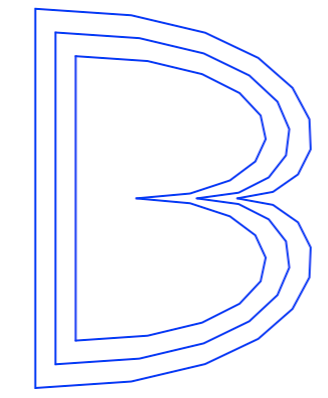
\includegraphics[width=0.25\linewidth]{BenInitial.png}
\caption{\label{fig:Ben}Ben's initial}
\end{figure}

\begin{figure}[h!]
\centering
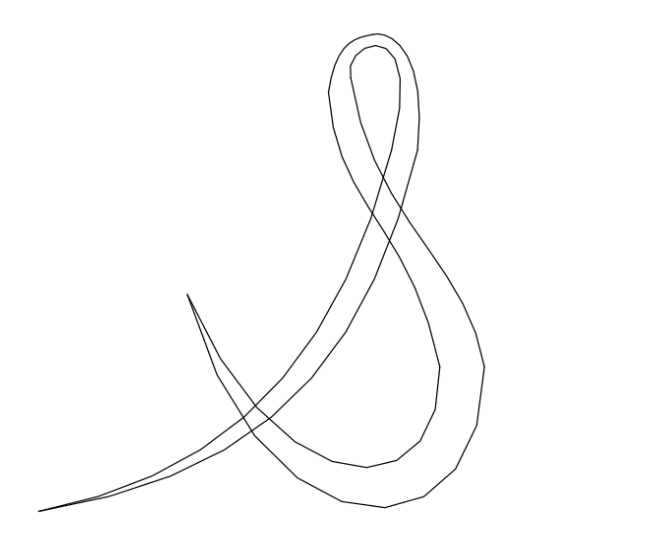
\includegraphics[width=0.6\linewidth]{S_initial.png}
\caption{\label{fig:Ben}Stan's initial}
\end{figure}

\newpage

\begin{figure}[h!]
\centering
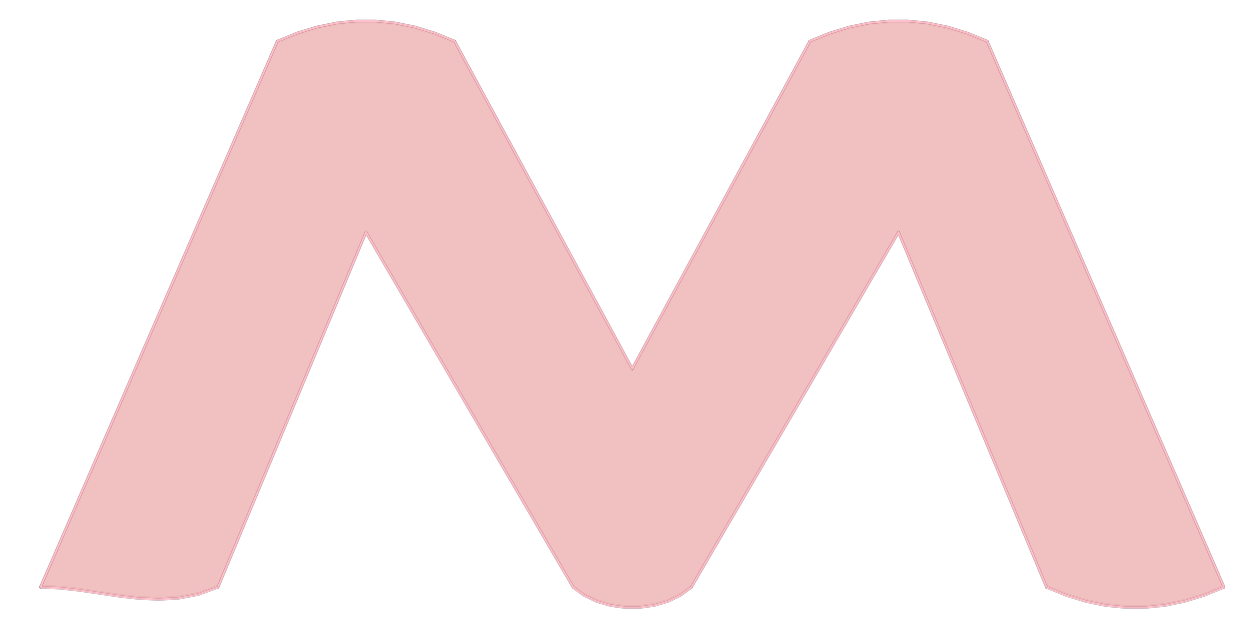
\includegraphics[width=0.5\linewidth]{M initial.png}
\caption{\label{fig:Ben}Mila's initial}
\end{figure}

Let's take the letter "M" as an example to illustrate how endpoints and control points function. The top left curved horizontal line of the letter "M" starts from the point (20, 100) and ends at (35, 100). These points define the beginning and end of the Bezier curve, serving as the coordinates of the endpoints.

\begin{figure}[h!]
\centering
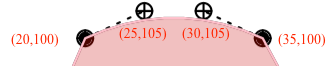
\includegraphics[width=0.5\linewidth]{Detail.png}
\caption{\label{fig:Ben}The top left curved horizontal line in M}
\end{figure}



However, to achieve the desired curvature, two control points are strategically and meaningfully positioned. These control points, located at (25, 105) and (30, 105), provide users with control over the slope at the endpoints of each spline. Essentially, they determine the slope of the endpoint within the spline. The Bezier curve links the endpoints while incorporating the slope of each endpoint, resulting in a curved line, as demonstrated in the figure 4.

We can also achieve straight lines using Bezier curves by aligning the control points with the endpoints, thus ensuring that the slope of the line remains consistent throughout. This concept is exemplified by the far-left line in Figure 4, where the starting point is (0, 0) and the ending point is (20, 100). Notably, both control points are set to (0, 0) and (20, 100) respectively, mirroring the endpoints.

\begin{figure}[h!]
\centering
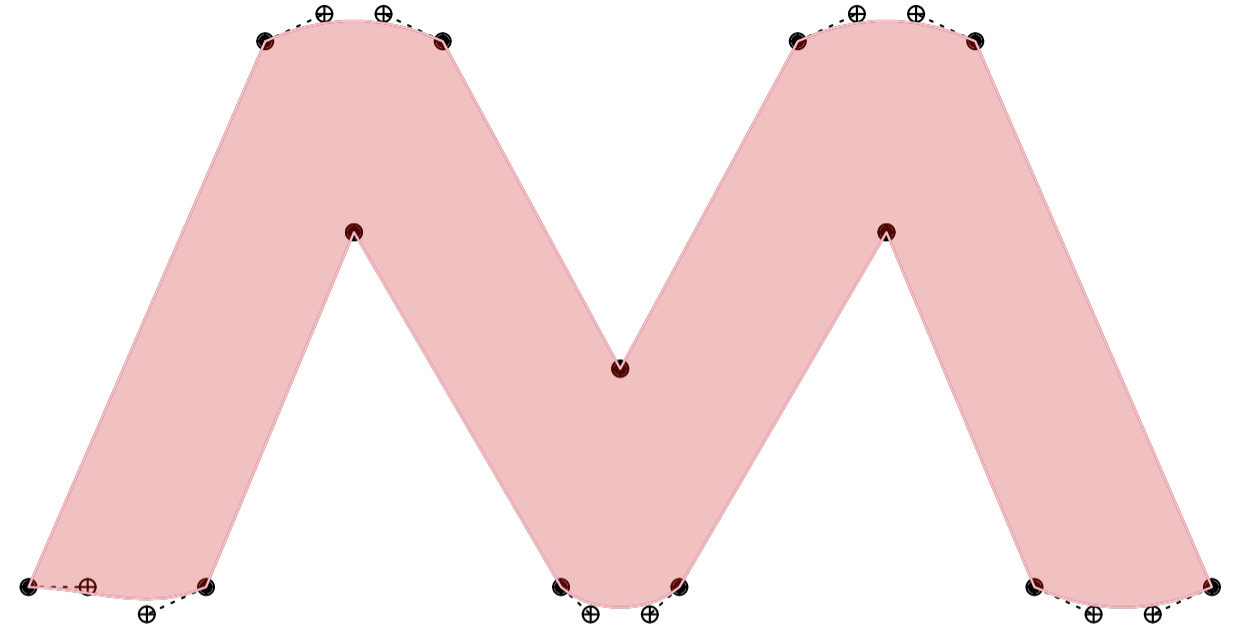
\includegraphics[width=0.5\linewidth]{M example.png}
\caption{\label{fig:Ben}Mila's initial with endpoints and control points}
\end{figure}

Hence, the fundamental approach to creating the letter involves designing multiple Bezier curves, each defined by its distinct set of endpoints and control points. By connecting these Bezier curves, the Capital Letter M emerges, adorned with colors.


\subsection{Helpful Hints}

When designing a letter with the provided bezier methods in R, the simplest way to approach is by first creating your vector variables and then calling those variables in the draw.beziers method to plot them all on the same graph. This approach can be seen in the code for the B initial and the S initial within the code appendix. When creating the vectors, here are a few hints to keep in mind to make the process a little bit easier:

\begin{enumerate}
    \item Each bezier curve that you plan on adding is associated with the same index for all of the vectors. For example, all of the first entries of the vectors for the 'B' initial correspond to the inner-most vertical bezier curve for the letter.
    \item For each curve, begin by adding the endpoints to the vector list first and then running the code to help you visualize before moving on to the control points to add any curvature. This means entering values for your vectors x1,y1 and x4,y4 first before filling out x2,y2 and x3,y3.
    \item In the plot functions within the draw.one.bezier and draw.beziers functions, adding in 'asp = 1' will set the aspect ratio of the plots to be 1:1 instead what they are originally set to by R's default settings. This will help to better center your letter while working and reduce overall distortion, making the entire process more intuitive.
    \item When you're all done with your letter, delete the 4 lines of code above the invisible method within the draw.one.bezier function to remove all the points and make your letter cleaner and more visible.
\end{enumerate}

\section{Conclusion}

In conclusion, Bezier curves can be used for font design because of the control that the user gets over the shape of the graph. There are infinite different styles that can be implemented as well as seen in the differences in the example letters seen in Section 2.2. However, a lot of information is needed to construct the plot of these letters, as each individual curve needs 4 points. Bezier curves are an interesting subset of cubic splines that can be effective of approximating functions and fitting data, and they have many applications to explore.

\bibliographystyle{alpha}
\bibliography{sample}

\bibitem{Ziegelmeier24}
  Lori Ziegelmeier,
  Activity 15,
  2024.

\vspace{2in}

\newpage

\section{Code Appendix}

\subsection{Code for B initial}

\begin{figure}[h!]
\centering
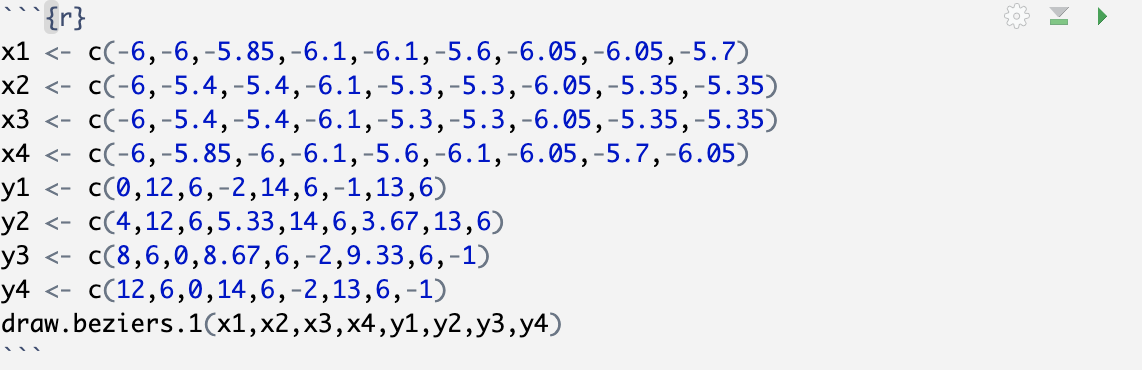
\includegraphics[width=5.5in]{BenCode.png}
\end{figure}

\subsection{Code for S initial}

\begin{figure}[h!]
\centering
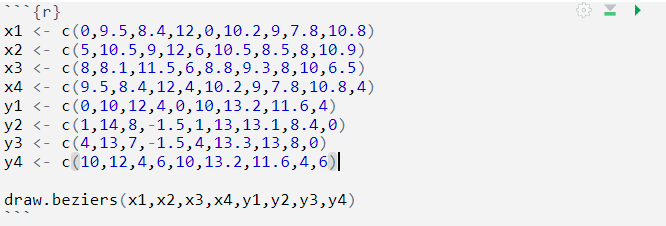
\includegraphics[width=5.5in]{s_code.png}
\end{figure}

\subsection{Code for M initial}
\begin{verbatim}
letter.M <- rbind(
  c(0, 0,0, 0, 20,100,20,100), 
  c(20,100, 25,105,30,105, 35,100),
  c(35,100,35,100,50,40,50,40),
  c(50,40,50,40,65,100, 65,100), 
  c(65,100,70,105,75,105,80,100),
  c(80,100,80,100,100,0, 100,0), 
  c(100,0,95,-5, 90,-5, 85,0), 
  c(85,0,85,0,72.5,65, 72.5,65),
  c(72.5,65,72.5,65,55,0,55,0),
  c(55,0,52.5,-5,47.5,-5,45,0),
  c(45,0, 45,0, 27.5,65,27.5,65),
  c(27.5,65, 27.5,65, 15,0, 15,0),
  c(15,0, 10,-5,5,0,0, 0,0))


draw.letter = function(T, npts = 10, ...) {
  pts = draw.beziers(T[, 1], T[, 3], T[, 5], T[, 7], T[, 2],T[, 4], T[, 6], T[, 8], npts = npts, ...)
  polygon(pts, col = rgb(0.8, 0, 0, 0.3),border="pink",xlab=" ",ylab=" ",)
}

draw.letter(letter.M)
\end{verbatim}



\end{document}